\documentclass{article}
\usepackage{spconf,amsmath,graphicx}

\usepackage{amssymb}
\usepackage{amsmath}
\usepackage{stmaryrd}
%\usepackage{pst-all}
\usepackage{graphicx}
\usepackage[all]{xy}
\usepackage{fancyvrb}



\usepackage{multirow}
\begin{document}
\renewcommand{\paragraph}[1]{{\bf #1}}
\newcommand{\comment}[1]{}

\title{FLIF: FREE LOSSLESS IMAGE FORMAT BASED ON MANIAC COMPRESSION}
\twoauthors
  {Jon Sneyers\thanks{Part of this research was performed while Jon Sneyers and Pieter Wuille were at
                      %the Department of Computer Science of 
                      the University of Leuven, Belgium,
                      and while Jon Sneyers was granted a fellowship of FWO-Vlaanderen (Research Foundation - Flanders).}}
	{Cloudinary Ltd.\\
	jon@cloudinary.com}
  {Pieter Wuille}
	{Blockstream\\
	pieter.wuille@gmail.com}


\maketitle

\begin{abstract}
We present a novel lossless image compression algorithm.
It achieves better compression than popular lossless image formats like PNG and lossless JPEG 2000.
Existing image formats have specific strengths and weaknesses: e.g. JPEG works well for photographs,
PNG works well for line drawings or images with few distinct colors.
%Our method has two main advantages:
%1) %the user does not need to know anything about the nature
%of the image and choose an image format accordingly, since
For any type of image,
our method performs as good or better (on average) than any of the existing image formats for lossless compression.
%2)
Interlacing is improved compared to PNG, making the format suitable for progressive decoding and responsive web design.
\end{abstract}
\begin{keywords}
Digital images, compression algorithms
\end{keywords}

\section{Introduction}

Lots of bandwidth and storage can be wasted by encoding images using a suboptimal file format.
For instance, a particular
image\footnote{This example refers to the 4000x4000 image {\tt Circos.ppm} from Niels Fr\"ohling's test set of sparse-color images.}
might need about 46 MiB when stored uncompressed.
If the user is sufficiently well informed, she will notice
that it is a line drawing with few different colors, % (28 to be precise),
so she saves the image as a GIF file (1106 KiB) or a PNG file (804 KiB),
%and perhaps she even uses a tool like {\tt pngcrush} to further reduce the size of the PNG file by a few kilobytes, or
or perhaps as a lossless WebP file (787 KiB).
If the user is not so well informed, he might save the image as a PNG24 file
(1.5 MiB), or much worse, as a lossy JPEG file (5.4 MiB), a lossy WebP file
(2.4 MiB), or a lossless JPEG 2000 file (12 MiB).%
\footnote{In case you are wondering: the FLIF file is 432 KiB.}
%Progressive decoding allows viewers to render a lower-quality preview while the compressed image
%stream is loading. This is particularly useful in low-bandwidth conditions.
%PNG and GIF support progressive decoding as an option, using interlacing.
%The interlacing of GIF happens only in the vertical direction, while PNG uses ``Adam7'' interlacing
%which works in two dimensions.
%However, this interlacing comes at a cost:
%in the case of GIF the file size goes up from 1106 kilobytes to 1122 kilobytes (an acceptable increase, but
%then again, GIF's interlacing is rather primitive); in the case of PNG, the file size increases
%more dramatically, from 802 kilobytes to 1146 kilobytes.
%an Adam7 interlaced PNG file is 1146 kilobytes (instead of 804 kilobytes non-interlaced).
%(Using our proposed image format, % (which we call FLIF, an abbreviation for ``Free Lossless Image Format''),
%the image is losslessly compressed to 432 KiB.) %, with lossless compression and progressive decoding (interlacing).

%Image formats like
Lossy formats like JPEG (2000), WebP and BPG %in lossy mode,
are great for photographs, but for other kinds of images,
the compression artifacts can be visible.
Image formats like GIF, PNG and lossless WebP work well for line drawings,
but they're less suitable for large photographs.
%but they only support lossless compression (and in the case of GIF, only 256 colors).
%
If 1) the image clearly belongs to one of these two categories (photograph / line drawing),
2) the user knows when to use which image format, %sufficiently aware of the properties of the different image formats, 
3) the user has the freedom to choose the format,
and 4) a single quality setting suffices for all use cases of the image,
then the existing formats are ``good enough'' in practice. However: %, these four conditions often do not hold together.

1) Many images are not photographs, nor line drawings, but something else or a combination of the two. For example, think of a poster that
contains a photo combined with text elements, %or the front page of a newspaper,
or a satelite image annotated with labels and arrows.
%,or a screenshot of a web browser.
%In these cases, the choice between, say, JPEG and PNG is hard: the artifacts of JPEG compression could
%be visible, while the PNG file could be too large. % (e.g. on the web, given limited bandwidth).

2) It is not easy to explain to non-technically oriented users when to use which image format (and which compression parameters).
It would be more user-friendly and less error-prone to have only one format that ``just works''.
%From the point of view of user-friendliness, it does not make sense that the user should worry about this. %the ``internal representation'' of her images.

3) Many devices, applications, and web services only support one (or a few) image formats.
As a result, sometimes users are forced to use suboptimal image formats.

4) Lossy compression by definition means that information is lost, and the sender of the image has to decide {\it how much} information
gets lost.
However, it is the receiver of the image who knows best what level of information loss (if any) is ``acceptable'' for their intended
use of the image.


We believe that the FLIF image format proposed in this paper can improve the state of the art.
New formats have been proposed in the past, but while improving the compression ratio, they kept the distinction between
two ``categories'' of images largely intact: e.g. JPEG 2000, lossy WebP and BPG improve upon JPEG,
while lossless WebP and PNG improve upon GIF.
In practice, at least two image formats are used and needed: e.g. on the web, JPEG and PNG are currently standard.
FLIF not just improves the compression ratio, but it also makes the old dichotomy obsolete:
FLIF works well for photographs {\em and} for line drawings, and everything ``in between''.


\section{Color Transformations}
\label{sec:color}

We assume an RGB(A) source image. % with integer RGB(A) color channels.
% and at most 16 bit depth per color channel.
%Our method can be extended to higher bit depths, floating-point pixel values and extra channels.
%
%The RGB color representation is well suited for image display on a computer screen, but it does not
%match the properties of the human eye.
Perceptually, luma (i.e. the grayscale image) is more important than color (chroma).
Lossy image compression aims to minimize perceptual error.
Most lossy formats use a luma+chroma color transformation, %space instead of RGB, 
%and they often use 
with
chroma subsampling
and/or quantization.
For lossless compression, color transforms are useful to
%decrease the correlation (and hence redundancy) between 
decorrelate
the color channels
%Also, while lossless compression by definition has no error, the perceptual error still matters for progressive decoding.
and to minimize perceptual error at intermediate steps of progressive decoding.
%
FLIF uses the reversible YCoCg color transformation of lossless JPEG 2000 \cite{JPEG2000}.
%
\comment{
Three popular color spaces are
RGB (red, green, blue), which is used in e.g. PNG and lossless WebP;
YCbCr (luminance, chroma blue, chroma red), which is used in e.g. JPEG and lossy WebP;
and YCoCg (luminance, chroma orange, chroma green), which is used in e.g. JPEG 2000 and FLIF.
Typical implementations of YCbCr are non-reversible (about two bits of information per pixel is lost),
while YCoCg is a reversible transformation.

We use the following transformation:
$$
\begin{array}{ccl}
Y & = & ((R+B)/2 + G)/2\\
Co & = & R-B \\
Cg & = & (R+B)/2 - G\\
\end{array}
$$
where the divisions are integer divisions.
Note that we convert three unsigned $k$ bit RGB values to one unsigned $k$ bit value (Y) and two $k+1$ bit values:
the Co and Cg values need an additional sign bit.


Since FLIF is lossless, all information has to be encoded, but in order to improve the perceptual quality of
progressive decoding, not all color channels are encoded at the same time.
The Y channel is most important, and will get priority over both the chroma channels.
We conjecture that the Co channel is perceptually somewhat more important than the Cg channel.
If an alpha channel is present,
it is considered even more important than the Y channel.
}


%\subsection{Bounds and Palette}
\paragraph{Bounds and Palette.}
Typically, an image only uses a small fragment of the full color space. We can improve compression by
taking that into account.
%For example, if the image is actually a grayscale image, the values for Co and Cg are always zero.
%
We record which values actually occur in each color channel. % (Y, Co, Cg, Alpha).
%, so every number that is outputted will be in that range.
The smaller the range of values, the fewer bits are needed to encode a number in the range.
For a singleton range %(i.e. a constant channel), 
no bits are needed at all.

%These global ranges only give a rough indication of the colors that occur: they only describe
%a bounding box in the three-dimensional color space.
%Photographic images typically use large continuous ranges of colors, but line drawings
%and other non-photographic images often use only a relatively small number of discrete colors.
Image formats like GIF and PNG can use a color palette
to encode sparse-color images concisely.
Their palette size is constrained since they encode pixels as (packed) bytes.
%If the total number of colors is low enough, it is a good idea to use a palette.
FLIF supports arbitrary palette sizes and
both 4-channel (YCoCgA) and 3-channel palettes (YCoCg), encoding the
alpha channel separately if needed.
The default maximum palette size is 1024 --- larger palettes rarely improve compression.

%If the image has a nontrivial alpha channel (i.e. it is not fully opaque), then
%FLIF first attempts
%to make a palette consisting of YCoCgA colors. If there are too many different YCoCgA colors, then FLIF
%will attempt to make a palette consisting of YCoCg colors, encoding the alpha channel separately.


%\subsection{Color Buckets}
\paragraph{Color Buckets.}
\label{sec:auto-indexing}
The palette approach only covers images which use a very small fragment of the full color space
(e.g. $2^{10}$ out of $2^{24}$ or $2^{32}$ possible colors).
%Some images contain a mix of continuous color ranges and discrete colors. For example, an
%image that contains a rendering of a document that contains both (anti-aliased) text and
%diagrams (e.g. generated by gnuplot)
%will typically use the entire grayscale range (256 colors) and a small number of non-gray colors.
%If the colored lines are also anti-aliased, then the total number of colors can quickly grow too
%big to be represented effectively using an indexed palette, but the image still only uses a relatively small
%fragment of the full color space.
We propose a simple yet effective mechanism, called {\it color buckets},
that generalizes the idea of color palettes. It works as follows.

For each value of Y, we keep track of the Co values that occur for that value. As long as the number of
distinct Co values for a given Y value is small, we maintain a list of discrete values (a ``discrete bucket'');
if that list becomes too large (according to some arbitrary threshold),
then we replace it by an interval, storing only the lower and upper bounds (a ``continuous bucket'').
Next, for each combination of Y and Co, we record the Cg values in a similar way.
To keep the total number of buckets reasonable, quantization is used and the mechanism is disabled
for high bit-depth images.

%Using this method, we get a ``color profile'' of the image.
%We will later make use of this profile to improve compression.
%in order to avoid writing redundant bits when outputting pixels.


%\subsubsection{Color Bucket Simplification}

%Obviously the decoder cannot compute the color profile from the original image; the
%color information has to be encoded so the decoder can load the information.
%Even when compressed, outputting the color table can be quite costly in terms of space (several kilobytes),
%and it may not always be worth it. We use a heuristic to decide whether to use color buckets.


%Photographic images typically use a rather large fragment of the total color space,
%and the color table will usually consist of a number of continuous buckets and a number
%of discrete buckets which contain a large amount of colors (close to the threshold).
%These discrete colors are usually not far removed from one another.

%The size of the color table can be reduced by converting discrete buckets to continuous
%buckets. We do this if the discrete bucket has at least 3 different colors and the volume of the
%bounding box of those colors is not much bigger than the size of the list.



\section{Image Traversal and Pixel Prediction}
\label{sec:traversal}

We have implemented two different methods to traverse the image.
The first method is a simple scanline traversal. %; it is %discussed in Section~\ref{sec:simple_traversal}.
%somewhat faster and easier to implement than the second one, but it is not suitable for progressive decoding.
The second method (the default method) is a generalization of PNG's Adam7 interlacing; it could be called ``Adam$\infty$ interlacing''.
It is somewhat more complicated and can result in slightly larger files, but it allows progressive decoding.
%This second method, which is FLIF's default method, will be discussed in Section~\ref{sec:interlacing}.

%Each color channel is encoded separately.
In both methods, the differences between predicted pixel values and actual values are encoded.
If the prediction is good, the differences are (close to) zero.

The differences can be positive or negative. At first sight, their range
is twice as large as the range of the original numbers. However, given the guess, only
half of that range is valid. Furthermore, not all YCoCg triples correspond
to valid RGB triples, further reducing the range.
The color buckets (if available)
are also used reduce the range and to snap the guessed value to a valid value:
if the relevant color bucket is discrete, the guess gets rounded to the nearest value in the list;
if it is continuous, then the guess gets clipped to the interval.
%This will be discussed in more detail in
%Section \ref{sec:rac:interval}.

\begin{figure}
\begin{center}
\begin{tabular}{|c|c|c|c|}
\hline
     &      & $TT$ & \\
\hline
     & $TL$ &  $T$ & $TR$ \\
\hline
$LL$ &  $L$ &   ?  &  $R$\\
\hline
     & $BL$ &  $B$ & $BR$ \\
\hline
\end{tabular}
\end{center}
\caption{Pixels around an unknown pixel indicated by `?'.}
\label{pixels}
\end{figure}


\paragraph{Scanline traversal (non-interlaced).}
\label{sec:simple_traversal}
The first traversal method is used in many image formats.
%, including non-interlaced PNG, non-interlaced GIF, WebP and FFV1.
The image is scanned line by line from top to bottom. Each line is scanned from left to right.
When outputting a pixel, the value of the pixels above and to the left are already outputted,
so those values can be used to compute a prediction that is also available at decode time (cf.\ Figure~\ref{pixels}).
%
As a prediction, we take the median of %the following three values:
$T$ (top), $L$ (left), and $T+L-TL$ (gradient).
This predictor is exactly the same as the one used in the FFV1 lossless video codec; it is a good guess if
the local area of the image happens to contain a smooth color gradient.




\paragraph{Adam$\infty$ Interlacing.}
\label{sec:interlacing}
The aim of interlacing is to be able to progressively reconstruct a compressed image, perhaps even
not loading the entire compressed stream if it is a large image and only a small preview is needed.
FLIF uses a generalization of PNG's Adam7 interlacing. In each interlacing step, the number of pixels
%roughly\footnote{exactly if it is a $2^n \times 2^m$ image}
doubles.

The first step is simply one pixel: the pixel in the top-left corner.
%Counting rows and columns from zero and from top to bottom, left to right, this is the pixel at position $(0,0)$.
Then, in each interlacing step, either the number of rows doubles (a horizontal step),
or the number of columns doubles (a vertical step). The final step is always a horizontal step, traversing all the
odd-numbered rows of the image.

%\paragraph{Pixel prediction.}
\label{sec:prediction_interlacing}
%There are two cases, which are similar up to rotation.
%In the case of a horizontal step, w
\comment{
In general, we have the following situation
(a horizontal step is shown here; vertical steps are rotated $90^\circ$) :
\begin{center}
\begin{tabular}{|c|c|c|c|c|}
\hline
$A$ & $B$ & $C$ \\
\hline
$P$ & $X$ &  \\
\hline
$D$ & $E$ & $F$ \\
\hline
\end{tabular}
\end{center}
}
In a horizontal step, $TL$, $T$, $TR$, $BL$, $B$ and $BR$ are known pixels (from a previous interlacing step), $L$ is also known
(it is the previous pixel in the current interlacing step).
As a prediction we use the median of: % the following three values:
the average of top and bottom $(T+B)/2$,
the top-left gradient $T+L-TL$, and
the bottom-left gradient $B+L-BL$.
%
In a vertical step we use the median of
%the average of left and right 
$(L+R)/2$ and
%the top-left gradient 
$T+L-TL$ and
%the top-right gradient 
$T+R-TR$.

\comment{
In a vertical step, $TL$, $L$, $BL$, $TR$, $R$ and $BR$ are known from a previous interlacing step and $T$ is
previously outputted in the current interlacing step.
As a prediction we use the median of: % the following three values:
the average of left and right $(L+R)/2$,
the top-left gradient $T+L-TL$, and
the top-right gradient $T+R-TR$.
}
%The top-left gradient is also used in the scanline traversal method, but the other two values are based on pixels $D$ and $E$ which
%would not be known during decoding in the scanline traversal method.
%
\comment{
In the case of a vertical step, we have the following situation in general:

\begin{center}
\begin{tabular}{|c|c|c|c|c|}
\hline
$A$ & $P$ & $D$ \\
\hline
$B$ & $X$ & $E$ \\
\hline
$C$ &     & $F$ \\
\hline
\end{tabular}
\end{center}

where $A$, $B$, $C$, $D$, $E$ and $F$ are known pixels (from a previous interlacing step), $P$ is also known
(it is a pixel outputted in the current interlacing step), and $X$ is
the pixel to be outputted.

We use as a prediction for $X$ the median of these three values:
\begin{itemize}
\item the linear interpolation between left and right: $(B+E)/2$
\item the top-left gradient $P+B-A$
\item the top-right gradient $P+E-D$
\end{itemize}
}
%
%The gradients can get a value outside the valid range, %:
%e.g. if the range is $[0,255]$ then the gradient can get a value as large as $510$ and as low as $-255$.
%In the case of scanline traversal, this is not an issue because we take a median of two actual pixel values and
%one gradient, so the median will always be inside the valid range. This is no longer the case with this predicted value:
%e.g. with $B=E=P=255$ and $A=D=0$ we would take the median of $255$, $510$ and $510$, which is $510$.
%so the prediction is clipped to the valid range.
% --- taking into account the global bounds and the color buckets, if available.



\paragraph{Channel Ordering.}
So far, we have only considered a single color channel. % of pixel values, i.e. a grayscale image.
When using scanline traversal, we simply process all the channels one by one:
first the alpha channel (if there is one),
then the Y channel, then the Co channel, and finally the Cg channel.
If the alpha value of a pixel is zero, then the pixel is completely transparent
and its values in the other channels are irrelevant.%
\footnote{At least, that is our opinion.
%One can also argue that the alpha channel
%masks parts of an image but the original ``behind the mask'' should be kept intact. %, even when pixels are completely masked.
For those with a different opinion,
there is an encoder option ({\tt -K}) to keep the color of fully invisible pixels intact.}
For this reason, the alpha channel is outputted first and the other channels are only encoded where the alpha value is nonzero.%
\footnote{
Still, those ``irrelevant'' pixels need to get Y, Co and Cg values, because they can be needed to predict other pixels.
Interpolation is used.
\comment{
Also, % as a more practical consideration, the %output formats to decompress to (e.g. PNG or PAM)
decompressed output
needs all pixels to have values for all channels.
In the case of scanline traversal, we replace the Y,Co,Cg values of $A=0$ pixels by their prediction.
%This is well defined even though that prediction itself may refer to earlier $A=0$ pixels.
In interlaced mode % we replace the Y,Co,Cg values of $A=0$ pixels by the linear interpolation between the adjacent pixels (top-down or left-right)
we use
%the average of the adjacent pixels from the previous interlace step, 
$(T+B)/2$ or $(L+R)/2$.
}
}

In interlaced traversal, the different channels are interleaved in such a way that the alpha and Y channels
get encoded earlier at higher resolutions than the chroma channels. This implies that the preview images obtained by progressive decoding
are automatically chroma subsampled.


\section{Entropy Coding: MANIAC}
\label{sec:rac}

Arithmetic coding \cite{ArithmeticCoding}, also known as range encoding,
is a form of entropy coding based on a probability model for the encoded bits.
Inspired by the FFV1 codec \cite{FFV1},
we use a variant of context-adaptive binary arithmetic coding (CABAC).

We call our entropy encoding method
``meta-adaptive near-zero integer arithmetic coding''
(MANIAC).
It is {\it meta}-adaptive since {\it the context model itself}
is adapted to the data.
%By ``meta-adaptive'', we mean the combination of
%taking into account the output integer interval (see section~\ref{sec:rac:interval})
%and, most importantly, the dynamic context tree learning (see section~\ref{sec:context_tree}).


\subsection{Context-Adaptive Binary Arithmetic Coding}

In CABAC, the probability model is adaptive.
%Since we are working with bits, the probability distribution can be expressed with
%a single number.
%(we use 12 bits of precision, i.e. chances of the form $k/4096$).
Initially we start with an arbitrary chance (e.g. 50\%) for each bit.
After processing a bit, the chance is updated. The aim is to learn the actual
distribution from the observed past to hopefully better predict the future.
%The same chance updates can be done when decoding since the update is
%only based on previously outputted bits.
%
%The above describes adaptive binary arithmetic coding.
If we have additional context information, we can use a different probability in each context.
Correlation between the context %information and the distribution of the actual symbols
and the bits
leads to more accurate probabilities and better compression.
Obviously all context information has to be available at decode time.




%\subsubsection{Integer Encoding Given Interval}
\label{sec:rac:interval}

To encode integers in a near-zero interval,
an exponent-mantissa representation is used, with a different context for each bit position.
Our binarization is based on that of FFV1, with some improvements.
%
%Suppose we want to output a value $x \in [-a,a]$.
First we output a single bit to indicate if $x = 0$.
%whether $x = 0$ or $x \neq 0$.
Then we output the sign of $x$, followed by the exponent, i.e. the number of bits $e = \lceil \log(|x|) \rceil$ needed to
represent $|x|$. %, where $e \in [1,\log(|a|)]$.
The number $e$ is encoded in {\em unary notation} as $e$ 1 bits followed by one 0 bit.
We use different contexts for each of these exponent bits.
Finally we output the mantissa bits; the leading 1 is omitted. % since we already know the exponent.
Redundant bits are omitted.%
\footnote{
In general, suppose the value $x$ to be encoded is in the interval $[a,b]$.
If the interval does not contain zero, the zero-bit is omitted.
If the signs of $a$ and $b$ are the same, the sign-bit is omitted.
There can be a lower bound on the exponent, e.g. if $x \in [32,80]$ then
we know $e \geq 5$ so the first 5 exponent bits can be omitted. If the exponent has the largest
possible value (e.g. 6 if $x \in [32,80]$), then it does not need to be followed by a 0 bit.
Finally, in the mantissa, %some bit values may be impossible,
some bits may be implied,
e.g. if $x \in [32,80]$ and
$e=6$ (so $x \in [64,80]$), then the most significant bit of the mantissa
(the one for 32) cannot be 1 since that would give a lower bound $x \geq 92$.
%If one of the two bit values is impossible, the bit can be omitted.
}
%it is implied that the bit must have the other value so it can be dropped.





\subsection{Context Model}

In FFV1, quantized pixel differences are used as context information.
%If the current pixel is $X$, then the following known neighbor pixels are used to determine the
%context:
Referring to Figure~\ref{pixels},
the differences $L-TL$, $TL-T$, $T-TR$, $LL-L$, $TT-T$ are computed and quantized (using
a logarithmic scale).
For every combination of these 5 properties, a different context is defined.
In total, 7563 different contexts (per color channel) can be used. %in the ``large'' context model of FFV1.


%\subsubsection{Relevant Pixel Properties}
In FLIF,
the contexts depend on the image traversal order.

\noindent
\paragraph{Scanline traversal:}
we use the same 5 differences as in %the ``large'' context model of 
FFV1 (but without quantization),
and we also use the following extra properties:
%\begin{itemize}
%\item
the prediction itself (the median of 3 values);
%\item
a number indicating which of those 3 values was used;
%\item
%the value of the pixel in all of the other channels that are already known. % (at most three: A, Y, and Co)
and the pixel value(s) in the 0, 1, 2 or 3 previously encoded channels.
%\end{itemize}
%In total, for pixels in the alpha channel, there are 7 properties, for pixels in the Y channel there are 7 or 8 properties
%(depending on whether there is an alpha channel), for pixels in the Co channel there are 8 or 9 properties, and for pixels
%in the Cg channel there are 9 or 10 properties.

\noindent
\paragraph{Interlaced traversal:}
%The above two to five properties are also used in the interlacing mode. The five properties from the
%``large'' context model of FFV1 are also used for the alpha, Y and Co channels; for the Cg channel,
%$LL-L$ and $TT-T$ are omitted.
the above 7 to 10 properties are also used.
Additionally, one more property is used: the
difference between the two adjacent pixels from the previous interlacing step
($T-B$ in horizontal steps, $L-R$ in vertical steps).
%Referring to section~\ref{sec:prediction_interlacing}, this corresponds to $B-E$.

%In total, for pixels in the alpha channel, there are 8 properties, for pixels in the Y channel there are 8 or 9 properties
%(depending on whether there is an alpha channel), for pixels in the Co channel there are 9 or 10 properties, and for pixels
%in the Q channel there are 8 or 9 properties.

%Since the space and time complexity of encoding (and, to a lesser extent, decoding) is proportional to the number of properties,
%it makes sense to restrict the number of properties.
\comment{
This set of properties is more or less arbitrarily chosen.
In future work, we can imagine an extension of the format where a description of the properties is part of the encoding and
user-defined properties can be used.
}

\begin{figure}
%\begin{center}
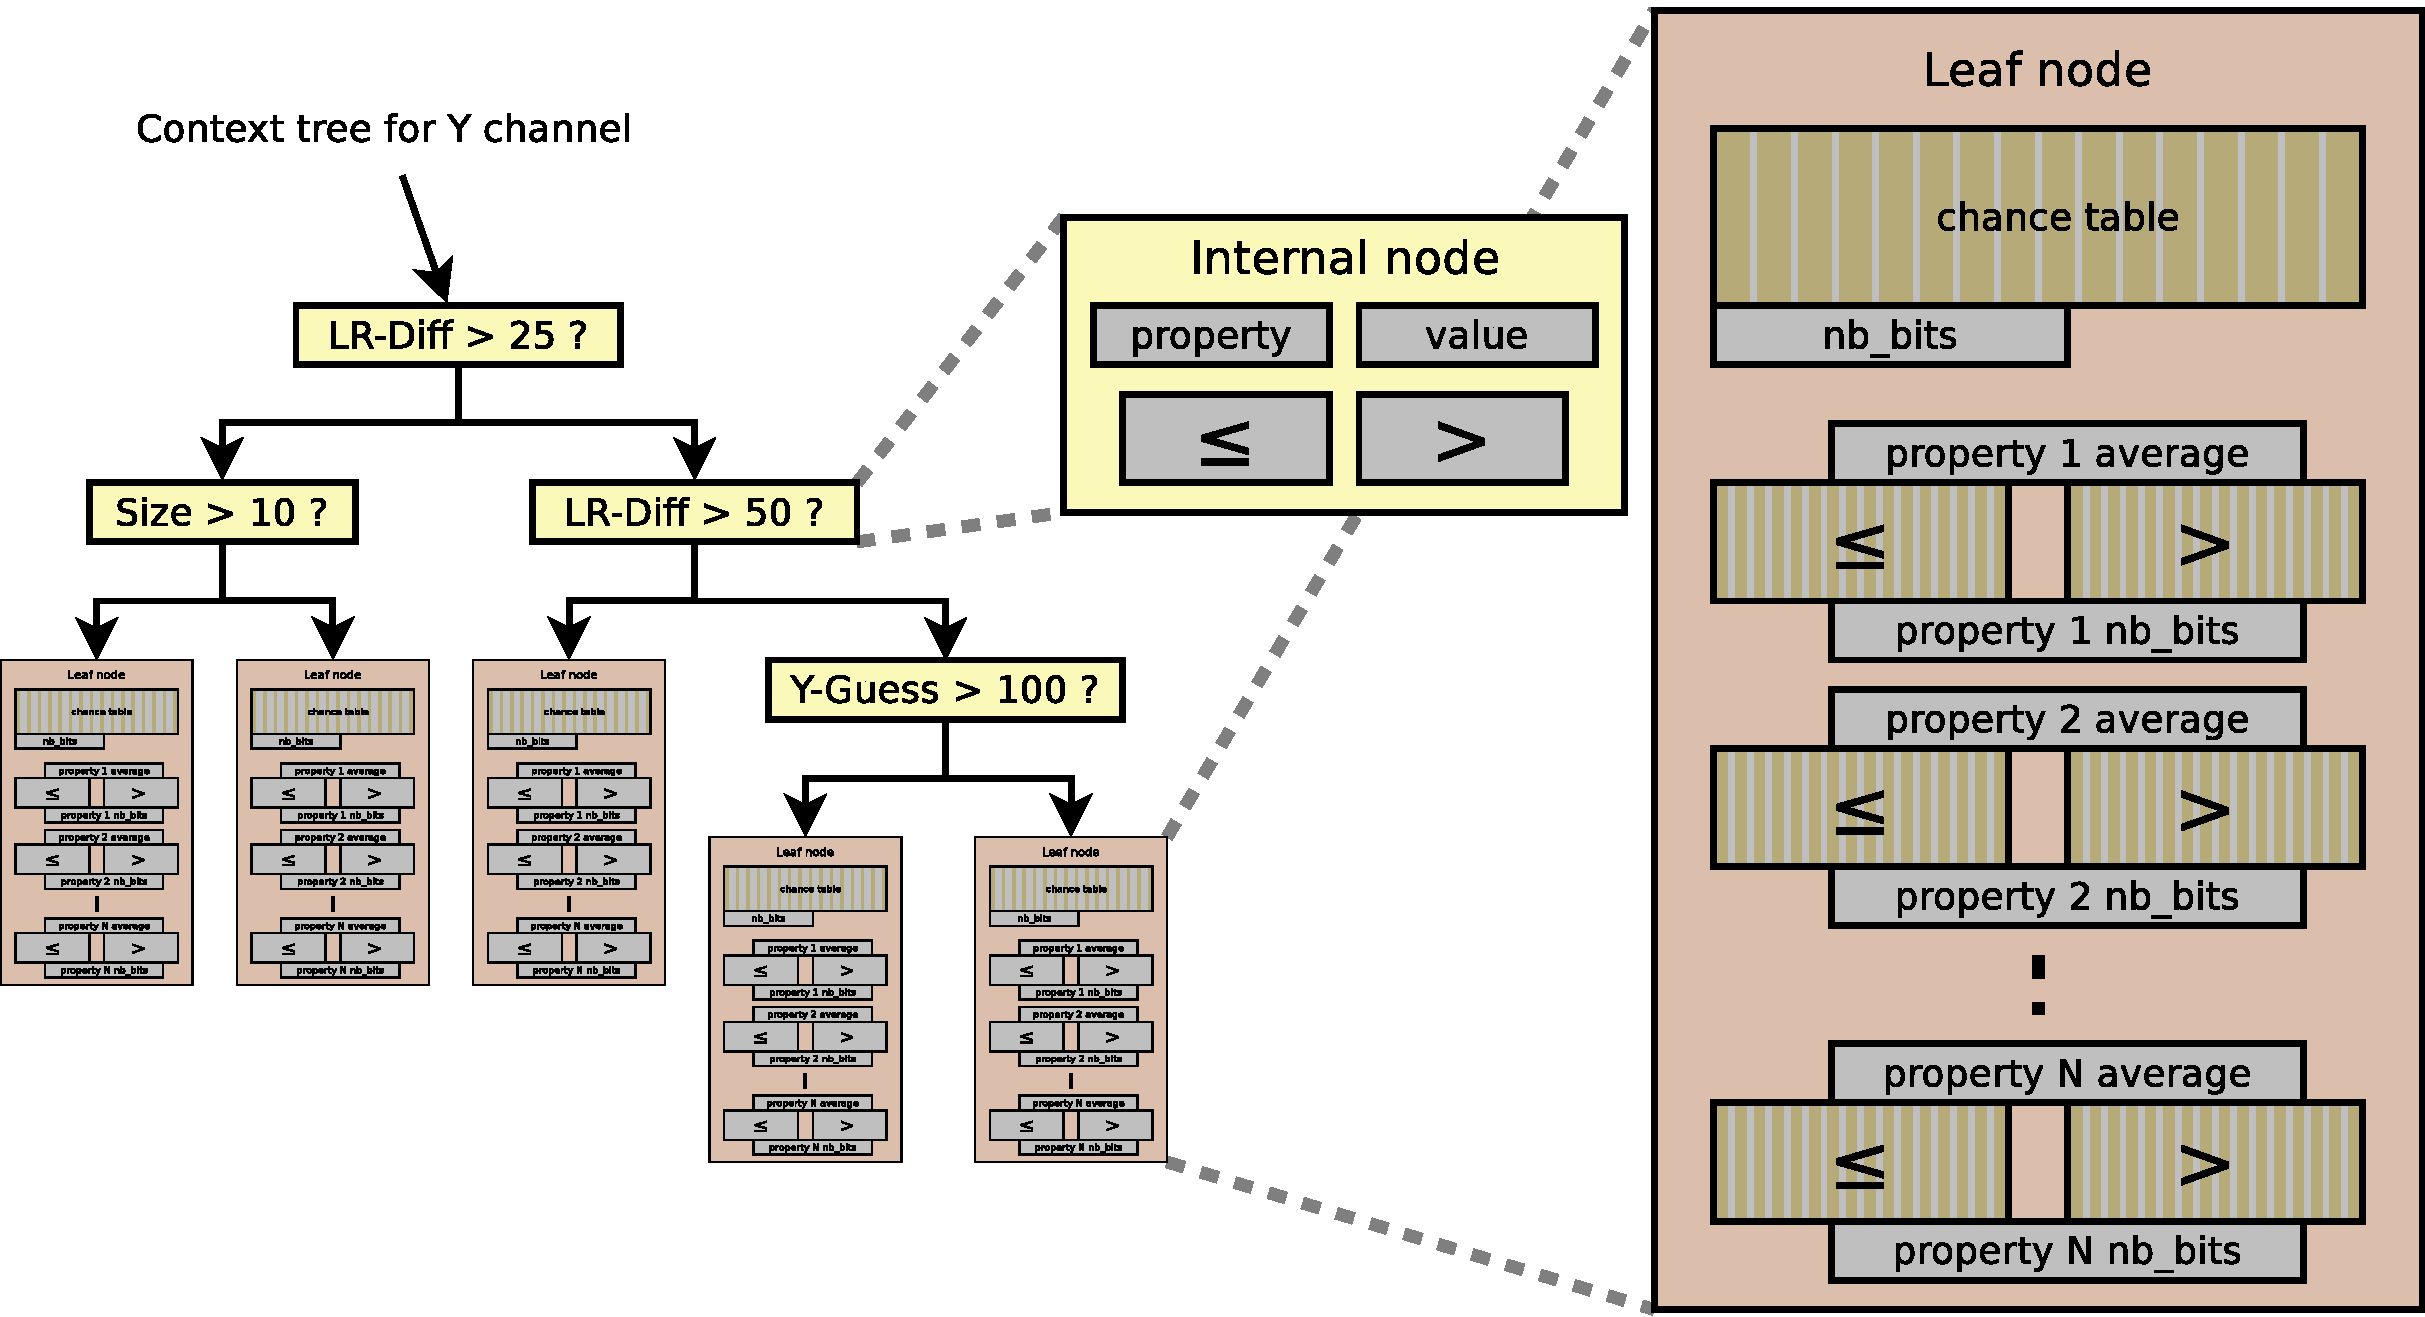
\includegraphics[width=\linewidth]{images/context_tree}
%\end{center}
\caption{MANIAC tree structure.}
\label{fig:context_tree}
\end{figure}

\subsection{MANIAC Tree Learning}
\label{sec:context_tree}

When using static contexts like in FFV1, where the number of contexts is the product of
domain sizes of each property, quantization has to be used in order to reduce
the number of contexts. It is hard to get the number of contexts ``just right'':
%On the one hand,
using too many contexts %consumes a lot of memory and also
hurts compression because context adaptation is limited
(few pixels per context);
%On the other hand,
but with too few contexts, compression also suffers
since pixels with different properties end up in the same context.
Also, when the contexts are defined statically,
a lot of the contexts are actually not used at all since the corresponding
combination of properties simply does not occur in the source image.




By contrast, we propose a dynamic data structure as a context model. It is essentially
a decision tree (actually one tree per channel), grown during encoding.
Figure~\ref{fig:context_tree} shows an example MANIAC tree.
%
Every internal (non-leaf) node has a test condition: an inequality comparing one of the context properties
to a value. The child nodes correspond to the two test branches.
During encoding, every leaf node contains one {\it actual} context (array of chances)
and two {\it virtual} contexts per property. %; at most 21 contexts in total ($1 + 2 \times 10$).
At decode time only the actual contexts are used.

\begin{figure}
%\begin{center}
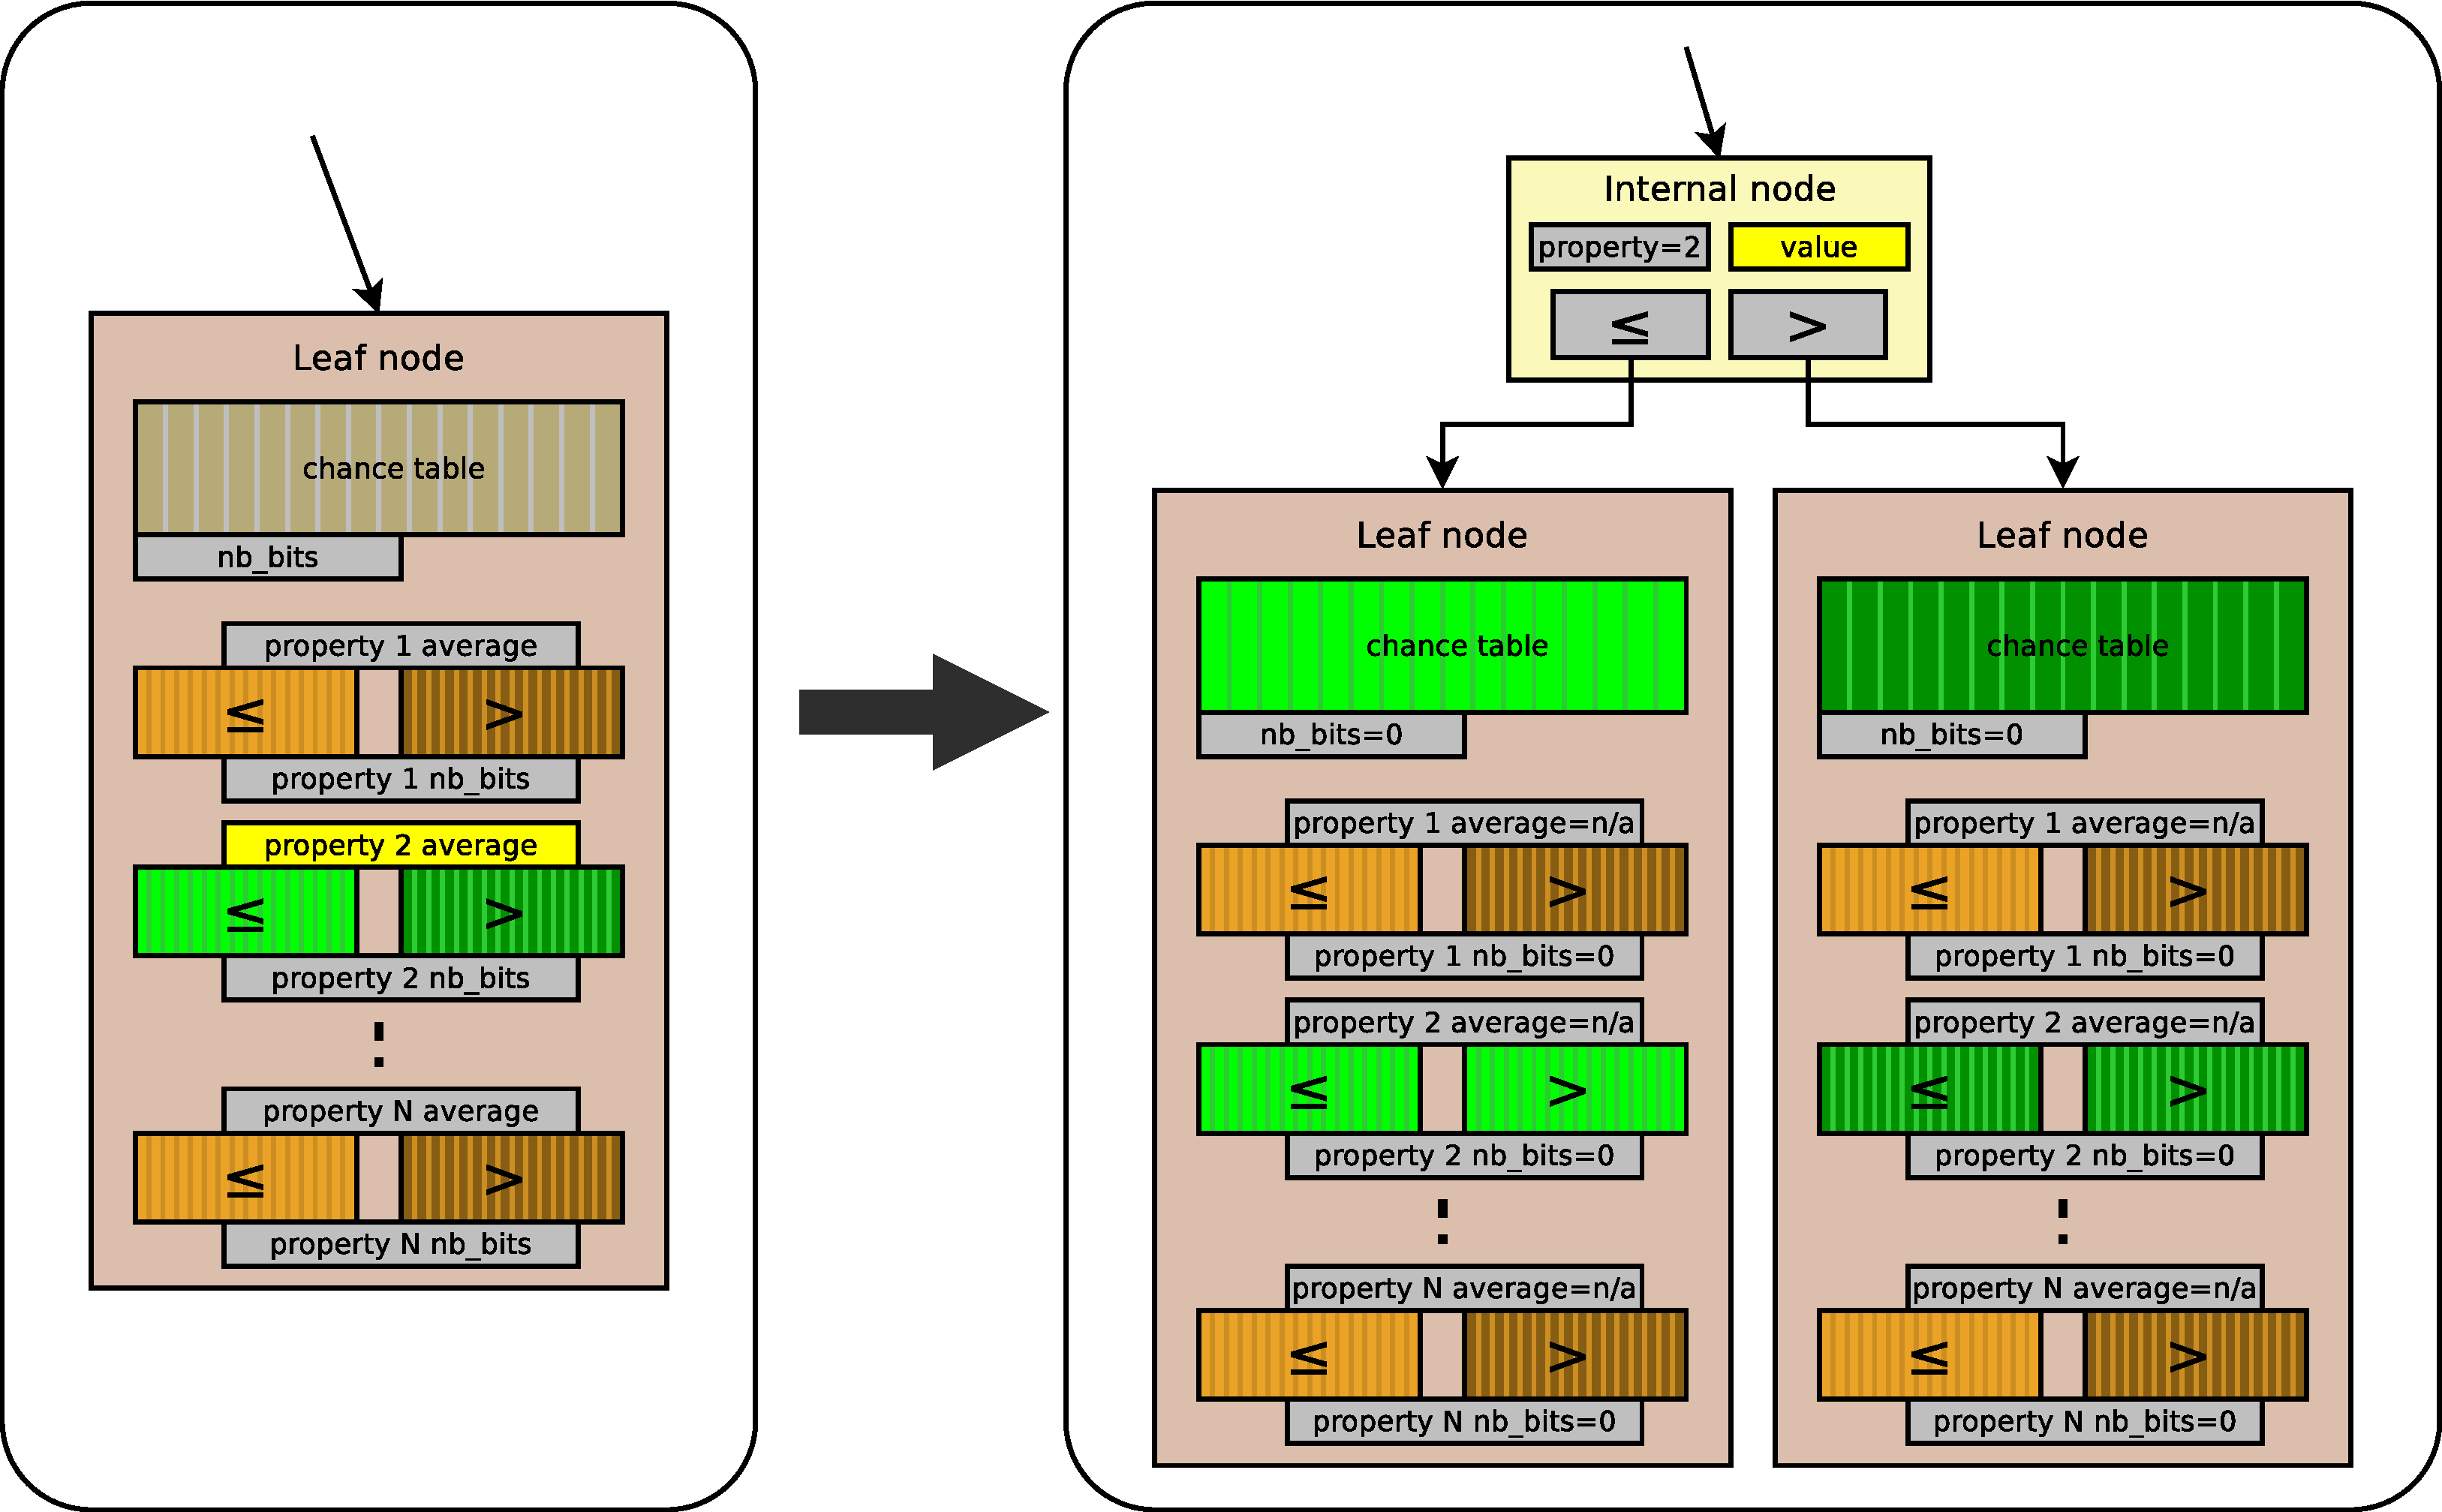
\includegraphics[width=\linewidth]{images/context_split}
%\end{center}
\caption{Growing a MANIAC tree: one step.}
\label{fig:context_tree_split}
\end{figure}


For each encoded value, the decision tree is traversed until a leaf node is reached.
Initially, the actual context is used to output the value, and a {\it cost estimate} (number of bits for the compressed output) is updated.
For each of the properties, each leaf node maintains a running average of the property values encountered at that leaf;
one virtual context is used for values below the average, the other is used for higher-than-average values.
For each property we select the virtual context accordingly,
and we output the same value again, but only ``virtually'', that is,
nothing is written to the compressed file, but the chances and cost estimate are updated.



These cost estimates indicate which properties are most significant.
If a property is irrelevant, then the sum of the costs for its two virtual contexts will be the same
or higher than that of the actual context. If however a property is relevant, then using two different
contexts depending on the value for that property will result in better compression.
We compare the cost of the ``best'' pair of virtual contexts in a given leaf node with the
cost of the actual context.
%If it performs better than the actual context,
%we use those virtual contexts instead of the actual context for output, maintaining
%the actual context as if it was virtual.
If the cost difference %between the best virtual context pair and the actual context
gets larger than some fixed
threshold, the leaf node becomes a decision node testing the ``best'' property.
Figure~\ref{fig:context_tree_split} illustrates this.
%
The MANIAC tree that we end up with is not necessarily optimal%
%since it is constructed in a rather simplistic greedy way
; future encoders can use other algorithms % to construct MANIAC trees
since the structure of the tree is part of the encoded bitstream.

MANIAC trees have three main advantages compared
to using a fixed context array:
1) There is no need to used quantized property values, so we can distinguish near-identical property values;
2) Properties are only actually used if they contribute to better compression for the specific image;
3) The context tree %(so the total number of contexts) 
scales with the image:
%the amount of pixels that are outputted and the actual relevance of the properties:
for large, complex images, more contexts will be used than for small, simple images.


\comment{
%\subsubsection{Two-pass Encoding}
MANIAC tree learning can be done in a symmetric or asymmetric way. FLIF uses the asymmetric method.

In the symmetric method, encoding is done in a single pass. Trees are learned during encoding and do not need to be
part of the compressed file, since the decoder can construct the trees in the same way as the encoder -- all information
needed is available at decode time. As a result, encoding and decoding need roughly the same amount of time and space.

\comment{
The main drawback of dynamically learning a context tree instead of using static contexts,
is the extra computational overhead arising from having to maintain the virtual contexts.
In fact, instead of doing the arithmetic coding once per pixel, it has to be done
up to $k+1$ times per pixel (where $k$ is the number of properties):
once for the ``actual'' context and up to $k$ times for the ``virtual'' contexts. The space needed per context
(to store the chance table and the bitcounts) goes from $O(1)$ to $O(1+2k)$.
However, there is a simple way to avoid the additional complexity during decoding.
}

In the asymmetric method, encoding is done in two (or more) passes.
In the first pass(es), we do exactly the same as before, except no actual compressed output is written.
The context trees are constructed and at the end, the final context trees are saved to the compressed file,
after some post-processing to simplify them. The actual chances and bitcounts are not saved, only the structure of the tree,
that is, the test in each node (one number to represent the property to test, another number to represent the value to compare to),
and also the number of times the node was visited as a leaf node, before it was ``split'' and became a decision node.\footnote{
This counter will be used to simulate the gradual reconstruction of the tree. Considering the tree as completely built from the start
leads to worse compression because then the chance tables are not initially shared and partially converged. However it does make sense
to make the counter smaller than its actual value (in the current implementation we divide it by a constant) because we already know
that the test ``will become useful in the future'' so it makes sense to ``split early''.}
In the second (last) pass, we consider the context trees
from the first pass(es) as given and proceed with normal encoding,
except that the context tree is already constructed so virtual contexts do not have to be maintained.
During decoding the context trees are read from the compressed file and decoding is quicker
because again there are no virtual contexts to maintain.

The compressed files can get slightly bigger than before
because we have to store the context trees and because we can no longer
use the best virtual context if it is better than the actual context.
However, the difference in compressed file size is relatively small while the
speedup for decoding can be significant.
Also, compression can be better if multiple passes are done, because that can lead to a better tree.
On typical images the cost of explicit trees is more than compensated by the gain from being able to use better trees.
}



\section{Experimental Evaluation}
\label{sec:benchmarks}


\begin{figure}
\footnotesize
\begin{center}
\setlength\tabcolsep{1.7pt} % default value: 6pt
\begin{tabular}{lcc|c|c|c|c|c|c|c|c|c|c}
\multicolumn{3}{l|}{Corpus} & \multicolumn{8}{c|}{Lossless formats} & \multicolumn{2}{c}{JPEG*}\\
\multicolumn{3}{r|}{\scriptsize (bit depth)} & FLIF & FLIF* & WebP & BPG & PNG  & PNG* & JP2* & JXR &\scriptsize  100\% &\scriptsize  90\%\\
\hline
\multirow{7}{*}{\rotatebox{90}{\scriptsize Natural (photo)}}
& \cite{corpus_testimages} & \scriptsize 8 & \bf 1.000 & 1.044  & 1.230 & 1.759 & 1.475 & 2.101   & 1.248 & 1.670 & \scriptsize 1.050 & \scriptsize 0.300 \\
& \multicolumn{2}{r|}{\cite{corpus_testimages}  \scriptsize 16} & 1.011 & 1.012 & / & / & 1.397 & 1.484 & \bf 1.000 & 1.986 & / & /\\
& \cite{corpus_kodak}      & \scriptsize 8 & 1.022 & \bf 1.000 & 1.085 & 1.584 & 1.403 & 1.633 & 1.077 & 1.225 & \scriptsize 0.999 & \scriptsize 0.297 \\
& \cite{corpus_wikipedia}  & \scriptsize 8 & \bf 1.000 & 1.020 & 1.034 & 1.329 & 1.272 & 1.430 & 1.065 & 1.158 & \scriptsize 0.972 & \scriptsize 0.261 \\
& \cite{corpus_icip-core1} & \scriptsize 8 & \bf 1.000 & 1.016 & 1.061 & 1.481 & 1.338 & 1.620 & 1.077 & 1.221 & \scriptsize 0.987 & \scriptsize 0.265 \\
& \cite{corpus_Lukas-2D} & \scriptsize 8 & \bf 1.000 & 1.018 & 1.057 & 1.227 & 1.135 & 1.362 & 1.073 & 1.289 & \scriptsize 1.148 & \scriptsize 0.381 \\
& \multicolumn{2}{r|}{\cite{corpus_Lukas-2D}  \scriptsize 12} & \bf 1.000 & 1.007 & / & 2.121 & 2.024 & 2.344 & 2.854 & 4.952 & / & /\\
\hline
\multirow{6}{*}{\rotatebox{90}{\scriptsize Artificial}}
%& \cite{corpus_renders} & \bf 1.000 & 1.007 & 1.124 & 1.187 & 1.293 & 1.399 & 1.198 & 1.527 & \scriptsize 0.898 & \scriptsize 0.130 \\
& \cite{corpus_fractals} & \scriptsize 8 & \bf 1.000 & 1.028 & 1.168 & 1.229 & 1.349 & 1.547 & 1.381 & 1.733 & \scriptsize 1.147 & \scriptsize 0.224 \\
& \cite{corpus_cartoons} & \scriptsize 8 & \bf 1.000 & 1.150 & 1.401 & 4.003 & 1.896 & 2.500 & 4.228 & 7.685 & \scriptsize 5.101 & \scriptsize 2.342 \\
& \cite{corpus_testimages-pattern-8bit}  & \scriptsize 8 & \bf 1.000 &  1.117 & 2.003 & 24.73 & 2.695 & 3.058 & 10.61 & 34.24 & \scriptsize 15.30 & \scriptsize 9.435 \\
& \cite{corpus_openstreetmap} & \scriptsize 8 & 1.072 & 1.186 & \bf 1.000 & 3.038 & 1.231 & 1.588 & 2.982 & 3.685 & \scriptsize 3.021 & \scriptsize 1.095\\
& \cite{corpus_PSF}           & \scriptsize 8 & \bf 1.000 & 1.104 & 1.653 & 3.219 & 2.173 & 2.731 & 4.515 & 10.21 & \scriptsize 5.708 & \scriptsize 2.947 \\
\end{tabular}
\end{center}
* : Format supports progressive decoding (interlacing).\\
/ : Unsupported bit depth.

Numbers are scaled so the best (smallest) lossless format corresponds to 1.
\caption{Compressed corpus sizes using various image formats.}
\label{benchmarks}
\end{figure}




We have evaluated (the reference encoder of) FLIF
by comparing its compression density to that of other lossless image compression algorithms
(PNG \cite{PNG}, JPEG 2000 \cite{JPEG2000}, JPEG XR \cite{JPEGXR}, WebP \cite{WebP},
BPG \cite{BPG}) % (which all have a lossless mode),
and to lossy JPEG \cite{JPEG} at maximum quality\footnote{
Even at 100\% quality, JPEG is lossy since its YCbCr transform reduces the number of
possible colors from $2^{24} = 16\,777\,216$ to only $4\,007\,551$.}
and at 90\% quality.
To optimize non-interlaced PNG files, we used ZopfliPNG \cite{ZopfliPNG};
for Adam7 interlaced PNGs, we used OptiPNG \cite{OptiPNG}.
For the other formats we used default lossless encoder options.
Figure~\ref{benchmarks} shows the results; see \cite{flif_benchmarks} for more details.

%We will also compare ``lossy'' partial decodings of interlaced FLIF files
%with progressive JPEG, progressive JPEG 2000, Adam7 interlaced PNG and interlaced GIF.
%Finally we evaluate the time and space complexity of encoding and decoding.
For one corpus (16-bit photographs), JPEG 2000 performed best; for one corpus (geographic maps), WebP was the best format.
For all other corpuses, FLIF was the (sometimes very clear) winner.
The difference between its interlaced and non-interlaced mode is typically small.

In terms of encoding/decoding speed, (our implementation of) FLIF is somewhat slower than the other formats.
This is explained in part by the inherent computational complexity of the algorithm, and in part by our implementation
lacking low-level (hardware-specific) optimization. It is however fast enough for most practical applications.

The reference FLIF encoder \cite{flif_website, flif_implementation}
is released under the terms of the GNU LGPL version 3 or later;
the reference decoder is available under the Apache 2.0 license.


\section{FLIF and Responsive Images}
\label{sec:conclusion}

%We have presented FLIF, a new image compression algorithm based on MANIAC entropy encoding.
%It outperforms standard compression algorithms like JPEG (2000) and PNG for lossless and near-lossless
%compression.
%; for medium-quality lossy compression of photographs, existing algorithms like JPEG 2000, WebP or BPG are still
%a much better choice.
Lossy image compression is useful when storage or bandwidth are limited.
Arguably, %at the time of writing (2016), 
storage is becoming relatively ubiquitous, while bandwidth conditions
have become increasingly variable (both in speed and price).

Responsive Web Design (RWD) aims to deal with various viewing devices and bandwidth conditions.
The typical approach to responsive images
is a mostly server-side solution where for each image, multiple files are created at various resolutions and quality settings.

We propose an alternative client-side approach, based on a single FLIF file per image.
Progressive decoding (i.e. partial downloading) allows fine-grained control over the desired
trade-off between image quality and transfer time and cost.
This trade-off depends on the receiver and their intention:
a quick preview,
a closer look,
a high-quality print,
or further image processing without cumulative degradation.

\section{Conclusion and Future Work}

FLIF is good at losslessly compressing various kinds of images, not just photographs.
Based on Adam$\infty$ interlacing and YCoCg interleaving,
its advanced progressive decoding
reduces the need for lossy compression.
We hope that FLIF can be a step in the direction of a `universal' image format.

MANIAC can be generalized to general-purpose compression.
%it uses data-dependent context properties in such a way that
%relevant properties are automatically exploited and irrelevant properties are ignored.
%
The underlying idea is to use machine learning to determine the most relevant features to construct the context model.
Many machine learning techniques could be used; we have used relatively simple decision trees, but any kind of classifier could be used.
Learning does not necessarily have to be fast --- encoding time is usually much less important than decoding time.
The only requirement is that the learned object (e.g. the decision tree) can be stored concisely and
that it can be reconstructed quickly during decoding.


\comment{

\subsection{Main Contributions}

MANIAC is a variant of arithmetic coding and can be applied not just to image compression. It is a general compression
method for integer numbers that are on average close to zero (e.g. differences between predicted and observed values).
MANIAC exploits all available information about the domain of the integers (e.g. in the case of FLIF, auto-indexing determines
the domain of the encoded integers). MANIAC also uses application-dependent context properties in such a way that
relevant properties are automatically exploited and irrelevant properties are ignored. Finally, because of
multiscaling, MANIAC automatically adjusts to the most appropriate time scale.

Some of the concepts used in FLIF are applicable more widely in other image processing and compression techniques.
We already mentioned MANIAC. Auto-indexing, a generalization of widely-used palette indexing, has many advantages compared
to traditional palette indexing. Most importantly, the combination of continuous and discrete color buckets means that no
arbitrary limit on the number of distinct colors has to be imposed, while the compression benefits of indexing can still be obtained.
Traditional palette indexing has the additional problem that the palette ordering heavily influences compression --- and since
the number of such orderings of $n$ colors is $n!$, exhaustive search for the optimal order is not feasible.
Auto-indexing does not have this problem; in this sense, it is more robust.




\subsection{Future Work}

The main idea behind the MANIAC is to use machine learning techniques to determine a relevant partitioning of the property space.
In a sense, we have used a very simple approach: we ``learn'' a decision tree (a rather simple kind of classifier),
where the learning is done in a very simple greedy way. More complicated classifiers and learning methods could be used.
Just like in the two-pass encoding mechanism,
learning does not need to be done on the fly. It does not necessarily have to be fast either --- encoding time is usually much less important
than decoding time. The only requirement is that the learned object (e.g. the decision tree) can be stored concisely and
that it can be reconstructed quickly during decoding.

Our current prototype only supports RGBA source images. In future work this should be extended to arbitrary data planes.
Our prototype does have preliminary support for animation; we will discuss this in a later paper.
Our choice to use YCoCg color decomposition needs to be evaluated experimentally in order to
compare its compression performance to that of other color decompositions.
}


\bibliographystyle{IEEEbib}
%\bibliographystyle{plain}
\bibliography{biblio}

\end{document}
